\section{Experimentos}

\begin{table}
\centering
\begin{tabular}{|l|l|l|}
\hline
          & \textbf{Simulated Annealing} & \textbf{Colonia de Hormigas} \\ \hline
{Escenarios probados} &       115                       &                              \\ \hline
{Solucionados} &                      70 (60\%)      &                              \\ \hline
{Dificultad baja} &                     71 \%         &                              \\ \hline
{Dificultad moderada} &                  40 \%            &                              \\ \hline
{Dificultad alta} &                         16\%     &                              \\ \hline
\end{tabular}
\end{table}

\subsection{Simulate annealing}
Para los experimentos elegimos un factor de enfriamiento en 0.5 y una temperatura inicial de 1. La justificación es en base a los experimientos realizados y que mostraremos en esta sección. \\ \\

El siguiente grafico es el resultado del tiempo que toma solucionar un Sudoku en donde partiendo de una solución existente blanqueamos celdas random y observamos como lo soluciona el algoritmo:
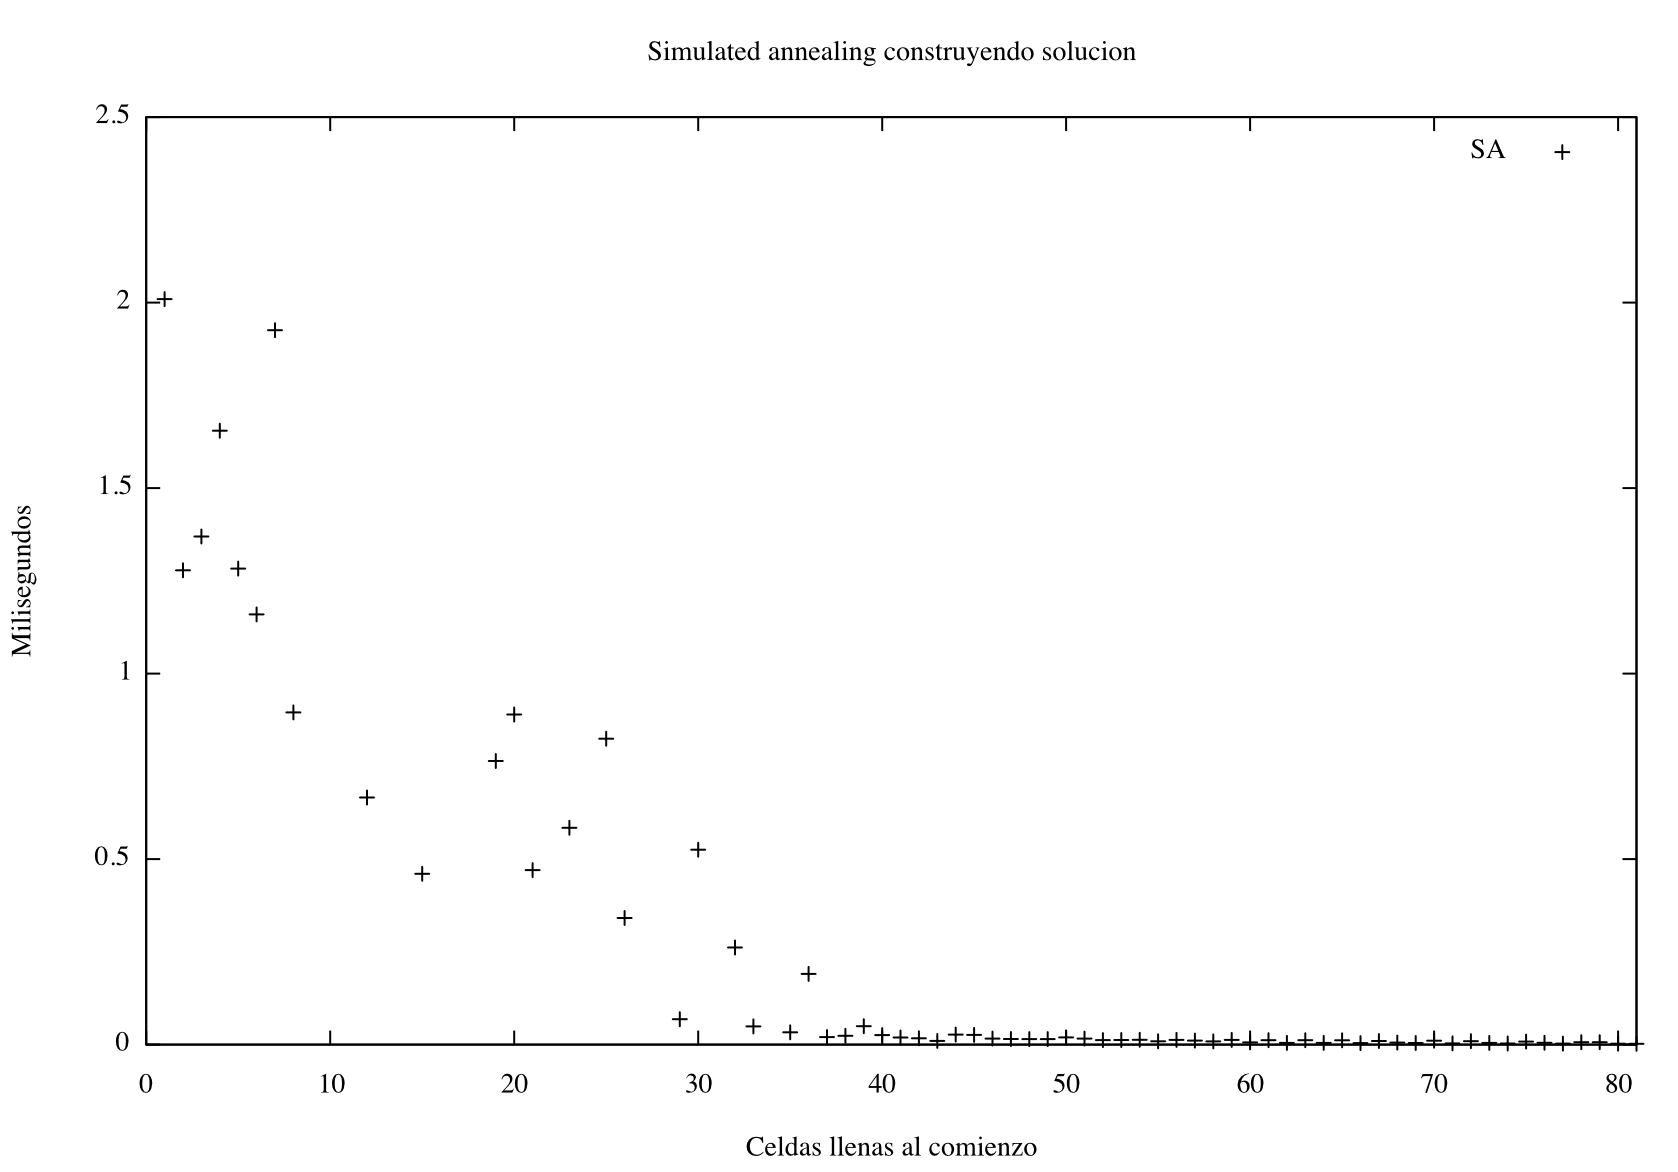
\includegraphics[scale=0.6]{imgs/randomSA.png}	
Clarmente se puede observar que a medida que el tablero esta mas lleno el tiempo es menor, eso es debido a la suma de varios factores, como que inicialmente infiere más celdas, son menos las vacias (que se convierte en menos iteraciones) y menos búsqueda de soluciones vecinas.\\\\

A continuación corrimos el algoritmo con 25 soluciones de diferentes niveles de dificultad, variando el factor de enfriamiento (o alfa):
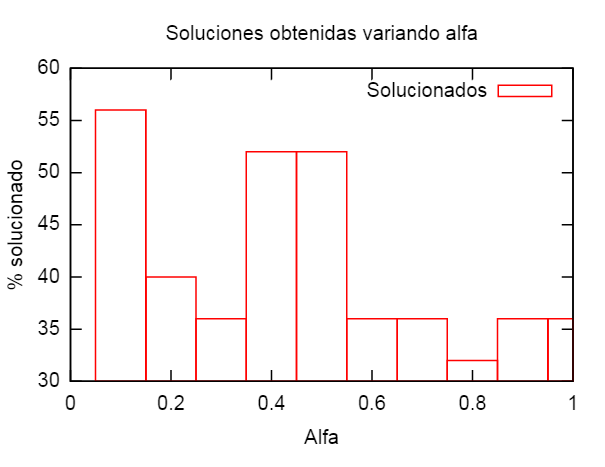
\includegraphics[scale=0.6]{imgs/porc_soluc.png}	
Si bien con valores intermedios (aprox 0.5) es donde se concentran las mejores soluciones, y que la mayor cantidad se logra con un 0.1, creemos en base a anteriores pruebas que el el factor de enfriamiento debería ser siempre mayor de 0.5 para que sea algo "lento" y no siempre elija ir por soluciones vecinas pero que tampoco las restrinja totalmente. 
